% =============================================================
%  AdapterSlots: IEEE Conference Format
%  Camera-ready
%  Compile: pdflatex final_paper_ieee && bibtex final_paper_ieee &&
%           pdflatex final_paper_ieee && pdflatex final_paper_ieee
% =============================================================
\documentclass[conference]{IEEEtran}

\usepackage{cite}
\usepackage{amsmath,amssymb,amsfonts}
\usepackage{amsthm}
\usepackage{algorithmic}
\usepackage{graphicx}
\usepackage{textcomp}
\usepackage{xcolor}
\usepackage{booktabs}
\usepackage{multirow}
\usepackage{microtype}
\usepackage{xspace}
\usepackage{enumitem}
\usepackage{xurl}
\usepackage[framemethod=default]{mdframed}
\usepackage[colorlinks=true,linkcolor=blue,citecolor=blue,urlcolor=blue]{hyperref}

% -- Theorem environments -----------------------------------------------
\newtheorem{theorem}{Theorem}
\newtheorem{proposition}{Proposition}
\newtheorem{definition}{Definition}

\surroundwithmdframed[
  backgroundcolor=blue!4!white,
  linecolor=blue!35!black,
  linewidth=0.7pt,
  roundcorner=3pt,
  skipabove=2pt, skipbelow=1pt,
  innertopmargin=2pt, innerbottommargin=2pt,
  innerleftmargin=4pt, innerrightmargin=4pt,
  nobreak=true,
]{theorem}

\surroundwithmdframed[
  backgroundcolor=teal!5!white,
  linecolor=teal!50!black,
  linewidth=0.7pt,
  roundcorner=3pt,
  skipabove=2pt, skipbelow=1pt,
  innertopmargin=2pt, innerbottommargin=2pt,
  innerleftmargin=4pt, innerrightmargin=4pt,
]{proposition}

\surroundwithmdframed[
  backgroundcolor=gray!6!white,
  linecolor=gray!50!black,
  linewidth=0.55pt,
  roundcorner=3pt,
  skipabove=2pt, skipbelow=1pt,
  innertopmargin=2pt, innerbottommargin=2pt,
  innerleftmargin=4pt, innerrightmargin=4pt,
]{definition}

% -- Custom commands ----------------------------------------------------
\newcommand{\asys}{AS\xspace}
\newcommand{\war}{\ensuremath{\mathrm{WAR}}\xspace}
\newcommand{\gwar}[1]{\ensuremath{\mathrm{GWAR}(#1)}\xspace}
\newcommand{\tmax}{\ensuremath{T_{\max}}\xspace}
\newcommand{\titer}{\ensuremath{\tau_{\rm iter}}\xspace}
\newcommand{\lora}{LoRA\xspace}

% =============================================================
\title{AdapterSlots: Warp-Aligned Multi-LoRA Serving\\
via WAR-Gated Kernel Promotion}

\author{
\IEEEauthorblockN{Shashank Tippanavar}
\IEEEauthorblockA{\textit{Dept. of Computer Science and Engineering} \\
\textit{IIIT Bangalore}\\
Bengaluru, India \\
shashank.tippanavar@iiitb.ac.in}
\and
\IEEEauthorblockN{Vivek Yadav}
\IEEEauthorblockA{\textit{Dept. of Computer Science and Engineering} \\
\textit{IIIT Bangalore}\\
Bengaluru, India \\
vivek.yadav@iiitb.ac.in}
}

% float packing: let a page carry more float area before spilling to the next
\renewcommand{\topfraction}{0.92}
\renewcommand{\bottomfraction}{0.85}
\renewcommand{\textfraction}{0.07}
\renewcommand{\floatpagefraction}{0.80}
\renewcommand{\dbltopfraction}{0.92}
\renewcommand{\dblfloatpagefraction}{0.80}
\setcounter{topnumber}{3}
\setcounter{dbltopnumber}{3}
\setcounter{totalnumber}{5}
\begin{document}
\raggedbottom

\maketitle

\begin{abstract}
Serving LLMs with concurrent per-request \lora adapters is a central
production-inference challenge.  The dominant batched \lora kernel, SGMV,
suffers operational intensity collapse as the number of active
adapters $K$ grows: mixing $K$ adapters can require $K{\times}$ as many distinct
adapter-weight loads and widens the throughput gap between adapter-aligned and
mixed batches to 78\% at $K{=}16$ (A6000, $N{=}2048$).
Nsight Compute profiling shows warp occupancy is unchanged at 8.33\% across all
mixing conditions, so the gap is not an occupancy effect; the dominant effect is
DRAM-bandwidth inflation ($3.07{\times}$ achieved DRAM throughput, fully-aligned
vs.\ fully-mixed).
We present \textbf{AdapterSlots (AS)}, a system that attacks this at two
levels.  At the scheduling layer, a per-adapter alignment buffer holds
decode tokens until warp-sized batches form, controlled by Erlang
fill-probability deadlines $T^*(k)$ and a PI controller that maintains a closed-loop
Warp Alignment Ratio (WAR) target under workload drift (14.3\,pp improvement over
a static policy), with a Whittle-inspired dispatcher that attains near-oracle
WAR at low per-tick cost (an $O(K\log K)$ index sort, measured below
200\,\textmu s for $K{\leq}128$).  At the kernel layer, \textbf{WAR-Gated Kernel
Promotion (WGKP)} uses the Generalized WAR metric $\gwar{n^*}$ as a runtime gate
to promote from SGMV to a fused Triton kernel ($\psi_{\rm fuse}{=}1.334{\times}$
at rank 16) or a merged-weight cuBLAS GEMM ($\psi_{\rm promote}{=}1.436{\times}$ at
rank 32), so that
alignment structurally drives throughput (Theorem~\ref{thm:causal}).
On a single RTX A6000, the full system achieves \textbf{1.525$\times$}
throughput over vLLM at $K{=}10$, rank=32 (mean of 3 independent runs;
CV=0.77\%).
On LLaMA-13B we observe gains of \textbf{1.33$\times$--1.62$\times$} at
$K{\in}\{4,8,16\}$, increasing monotonically with adapter diversity.
Adapter-Partitioned Independent Serving (APIS) achieves \textbf{2.598$\times$}
at $K{=}50$ on two RTX A6000 PCIe.
\end{abstract}

\begin{IEEEkeywords}
multi-LoRA serving, warp alignment, SGMV, WAR-gated kernel promotion,
Erlang deadlines, Whittle-inspired dispatch, APIS
\end{IEEEkeywords}

\sloppy

% =============================================================
\section{Introduction}
\label{sec:intro}

Parameter-efficient fine-tuning via LoRA~\cite{hu2021lora} has transformed
production LLM serving: a single base model handles hundreds of fine-tuned
adapters concurrently~\cite{kwon2023vllm,yu2022orca}, each serving a distinct
user group or task domain.
The dominant kernel for concurrent multi-adapter execution is
SGMV~\cite{chen2024punica}, which batches each adapter's low-rank matrix
products into a segmented GEMM to amortise GPU launch cost.
The problem is that SGMV's efficiency degrades sharply as the number of active
adapters $K$ grows.
On NVIDIA RTX A6000 hardware, at $K{=}16$ the throughput gap between
fully adapter-aligned and fully adapter-mixed batches reaches \textbf{78\%}.

\textbf{Root cause: DRAM bandwidth inflation.}
A common assumption blames this gap on GPU warp divergence---threads
within a warp taking different execution paths.
Occupancy is not the mechanism: \texttt{sm\_\_warps\_active} is unchanged at
\textbf{8.33\%} across all four mixing conditions (fully aligned through fully
mixed).
The dominant measured effect is DRAM bandwidth inflation: mixing $K$ adapters forces
loading $K$ distinct weight sets, raising achieved DRAM throughput from
10.2\% to 31.3\% of peak---a $3.07{\times}$ increase (conditions A through D).

\textbf{The alignment opportunity.}
The fix is conceptually simple: hold each adapter's decode tokens in a small
buffer until a full GPU warp's worth ($W{=}32$ tokens) accumulates, then
dispatch them together.
Threads in the warp then operate on the same adapter weight set, substantially
reducing the redundant HBM traffic that adapter mixing induces.
The challenge is twofold: (1) computing per-adapter waiting deadlines that
are short enough to preserve tail latency, and (2) ensuring that a more
aligned batch actually runs faster---something prior systems do not guarantee.

\textbf{Prior systems do not close the loop.}
Punica~\cite{chen2024punica}, S-LoRA~\cite{sheng2023slora}, and
dLoRA~\cite{wu2024dlora} all try to group tokens by adapter but then hand the
batch to the same SGMV kernel regardless of how well-aligned it is.
As a result, alignment correlates with throughput only indirectly---because
fewer adapters means less mixing---never because the kernel exploits it.

\textbf{Our insight: use alignment to select the kernel.}
\asys introduces WAR-Gated Kernel Promotion (WGKP).
Instead of running SGMV unconditionally, \asys measures how well-aligned the
current batch is---using the Generalized WAR metric $\gwar{n^*}$---and
promotes well-aligned segments to progressively faster kernels.
This makes alignment a structural determinant of throughput rather than a
passive correlate (formalised in Theorem~\ref{thm:causal};
Fig.~\ref{fig:overview}).

\textbf{Contributions:}
\begin{itemize}[leftmargin=*,noitemsep,topsep=0pt]
\item \textbf{AlignmentBuffer}: per-adapter queues with Erlang-derived deadlines
  $T^*(k)$, a PI feedback loop that tracks WAR under workload drift (mean-square
  stable under an online-estimated gain bound), and a Whittle-inspired dispatcher
  that keeps overhead under 200\,\textmu s at $K{=}128$.
\item \textbf{WGKP}: a three-level kernel stack (SGMV / Fused Triton / merged
  cuBLAS GEMM) gated on $\gwar{n^*}$, with a proof that higher GWAR
  structurally raises throughput (Theorem~\ref{thm:causal}).
  Measured: $1.334{\times}$ at L2 (rank 16), $1.436{\times}$ at L3 (rank 32)
  over SGMV.
\item \textbf{APIS}: two TP=1 shards instead of PCIe TP=2, shrinking the
  per-shard scheduling interval from 100.4\,ms to 29.3\,ms and restoring the
  alignment budget.
\item \textbf{Hardware results}: $1.525{\times}$ on LLaMA-7B
  at $K{=}10$, 1$\times$\,RTX A6000 (CV=0.77\%); $1.33{\times}$--$1.62{\times}$ on
  LLaMA-13B~\cite{touvron2023llama} at $K{\in}\{4,8,16\}$; $2.598{\times}$ via
  APIS at $K{=}50$ (2$\times$\,RTX A6000 PCIe).
\end{itemize}

\begin{figure*}[t]
  \centering
  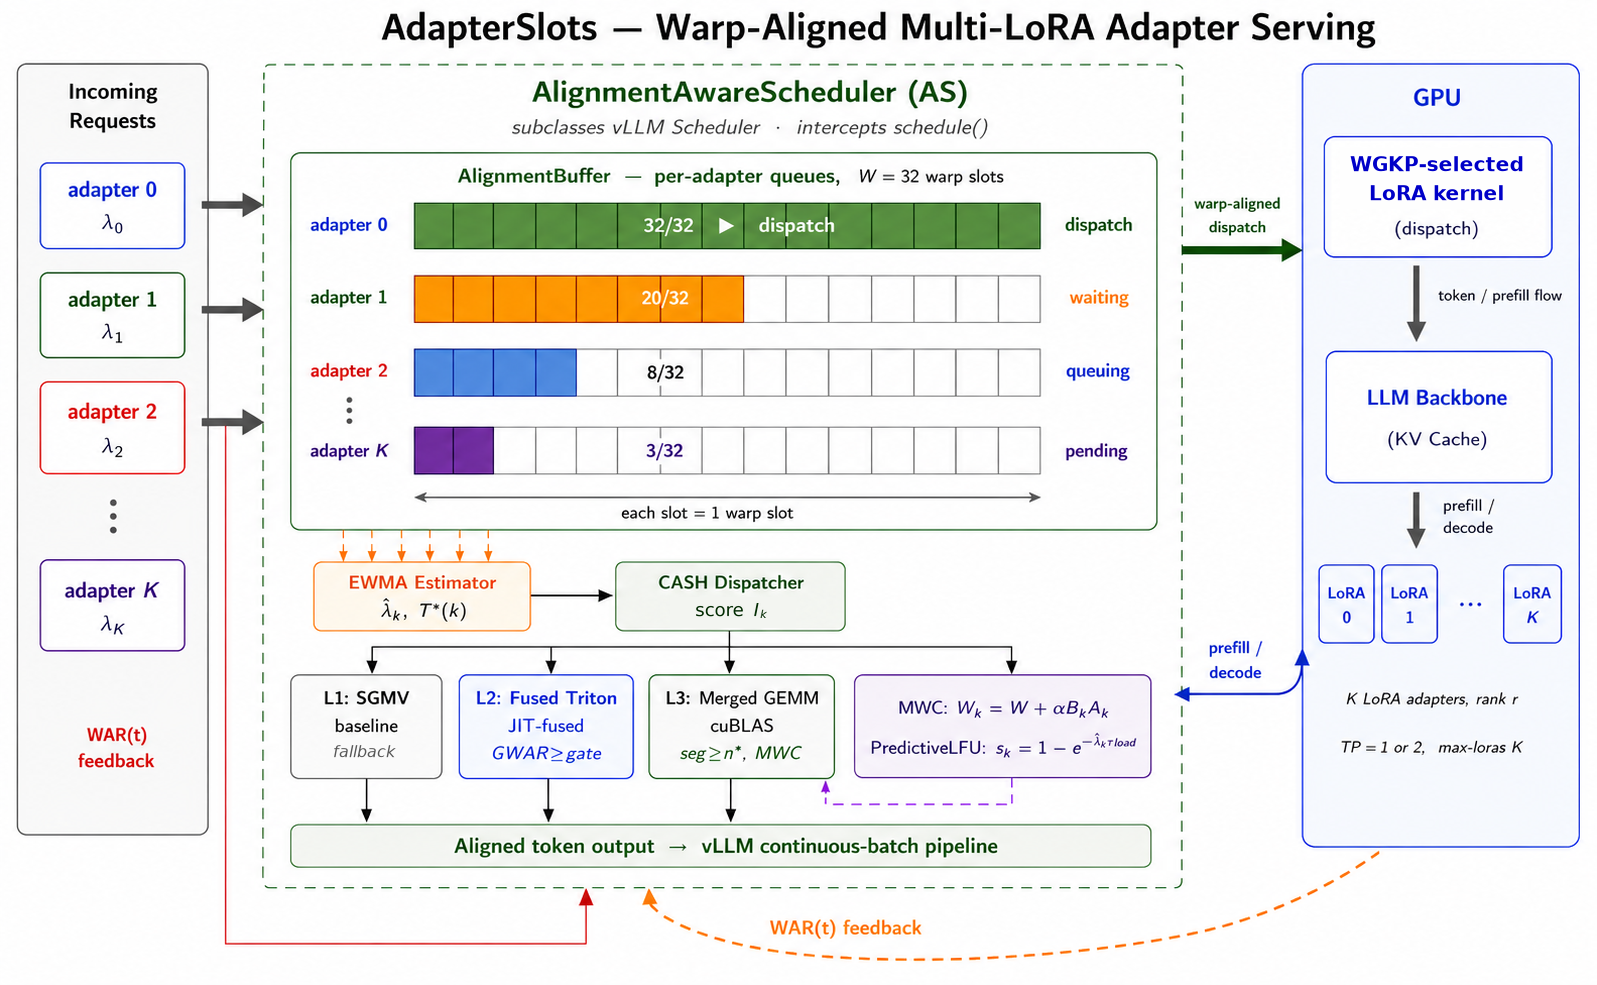
\includegraphics[width=0.63\textwidth]{final_figures/final_AS.png}
  \caption{AdapterSlots system overview.  Incoming requests are enqueued in
    per-adapter deques inside the AlignmentBuffer.  The EWMA estimator computes
    per-adapter token rates $\hat\lambda_k$ and Erlang deadlines $T^*(k)$;
    the CASH dispatcher (CASH score $I_k$) selects which queues to flush each tick.
    WAR feedback from the PI controller adjusts $T_{\max}$ under workload drift.
    WGKP gates dispatched segments into three kernel tiers: L1 SGMV (fallback),
    L2 fused Triton (GWAR ${\geq}$ gate), L3 merged cuBLAS GEMM
    (segment ${\geq}n^*$ and adapter in MWC).
    The Merged Weight Cache (MWC) pre-computes $W_k{=}W{+}\alpha B_kA_k$
    with PredictiveLFU eviction; aligned output feeds the vLLM continuous-batch pipeline.}
  \label{fig:overview}
\end{figure*}

% =============================================================
\section{Scheduling Stack: Generating the GWAR Signal}
\label{sec:buffer}

\textbf{SGMV intensity collapse.}
For adapter $k$ in a batch of $N$ tokens spread across $K$ adapters, the
SGMV operational intensity (tokens per weight-byte loaded) is proportional
to $N/(Khr)$, where $h$ is the hidden dimension and $r$ the LoRA rank.
As $K$ grows, each adapter gets fewer tokens per batch and the GPU must load
more distinct weight sets, collapsing memory efficiency.
Hardware profiling (NVIDIA Nsight Compute) shows achieved
DRAM throughput rising by over $3\times$ from a fully-aligned to a fully-mixed
batch at $K{=}4$.
Alignment buffering counteracts this: tokens accumulate per adapter and are
dispatched together as full warps.

\textbf{AlignmentBuffer.}
\asys maintains a per-adapter deque $Q_k$ inside the vLLM scheduler loop; after
each iteration's sequence selection, decode tokens for adapter $k$ are appended.
Dispatch fires when either condition holds:
\begin{equation}
|Q_k| \geq W \;\;\text{or}\;\; \mathrm{age}(Q_k) \geq T_{\max}^{(k)},
\label{eq:dispatch}
\end{equation}
where $W{=}32$ is the warp width: the queue is warp-full, or the per-adapter
deadline has expired.
The two controllers are alternatives for that deadline, capped alike: Erlang
mode sets it to $\min\{T^*(k),T_{\rm SLO}\}$ (Theorem~\ref{thm:erlang}), PI
control to $\min\{T_{\max}^{(t)},T_{\rm SLO}\}$ for one global $T_{\max}^{(t)}$.

\begin{definition}[WAR and GWAR]
\label{def:war}
Partition each dispatched batch into maximal contiguous same-adapter runs.
The Generalized WAR $\gwar{n^*}$ is the fraction of dispatched \emph{tokens} in
runs of length ${\geq}n^*$, indexed by the promotion threshold $n^*$; this is
what the WGKP gate consumes.  The Warp Alignment Ratio is the complementary
\emph{per-warp} measure: the fraction of the $\lfloor N/W\rfloor$ complete warps
that are adapter-homogeneous.  The denominators differ, so the two values are
not directly comparable.
\end{definition}

\textbf{Erlang fill-probability deadlines.}
One rate drives the controller: $\hat\lambda_k$, the rate at which decode tokens
accumulate in $Q_k$.  The EWMA estimator measures it from token inter-arrivals;
the inversion, the CASH score and APIS all consume that estimate.  A trace's aggregate \emph{request} rate, written
$\lambda$ without hat or subscript, never enters a deadline.
Under Poisson token arrivals at rate $\hat\lambda_k$ the time to accumulate $W$
warp slots is Erlang-$W$~\cite{erlang1917theory,kleinrock1975queueing}, whose CDF
inverts to the deadline achieving a target fill probability.

\begin{theorem}[Erlang fill-probability deadline]
\label{thm:erlang}
Let $F_{W,\hat\lambda_k}$ be the Erlang-$W(\hat\lambda_k)$ CDF and $T_{\rm SLO}$ a maximum-wait cap.  Timing accumulation from an empty $Q_k$, the per-adapter deadline
$T^*(k) = \min\{F^{-1}_{W,\hat\lambda_k}(\mathrm{WAR}^*),\;T_{\rm SLO}\}$
makes adapter $k$ fill a full warp before its deadline with probability exactly
$\mathrm{WAR}^*$ whenever the cap is inactive.
\end{theorem}

\begin{proof}
Poisson arrivals give i.i.d.\ exponential inter-arrival times; by convolution the
time to accumulate $W$ tokens from an empty queue is Erlang-$(W,\hat\lambda_k)$.
With the cap inactive, $F(T^*(k)) = \mathrm{WAR}^*$, so
$\Pr[T_{\rm fill} \leq T^*(k)] = \mathrm{WAR}^*$ by definition of the CDF.
Strict monotonicity of the Erlang CDF gives uniqueness, and bisection on the
regularised incomplete gamma function computes the quantile efficiently.
When the cap binds, $T^*(k) < F^{-1}(\mathrm{WAR}^*)$ and the attained fill
probability is $F(T_{\rm SLO}) < \mathrm{WAR}^*$.
\end{proof}

\textbf{Fill probability, rates, and the cap.}
Theorem~\ref{thm:erlang} concerns the \emph{probability} that a queue reaches a
full warp, not the per-warp $\war$ of Definition~\ref{def:war}: queues expiring
at the deadline still dispatch partial runs, so the realised $\war$ generally
differs from $\mathrm{WAR}^*$, which we therefore treat as a control set-point
while measuring $\war$ directly throughout.
The scoping matches the implementation: the buffer times each queue from its
empty-to-nonempty transition, so every cycle starts at zero and no residual
Erlang-$(W{-}s)$ term arises.
The Erlang-$W$ CDF depends on rate and deadline only through their product, so
attained fill is a function of $\hat\lambda_k T^*(k)$ alone: one dimensionless
constant ($36.638$ at $W{=}32$, $\mathrm{WAR}^*{=}0.8$) fixes the family, and a
check at one rate is a check at every rate.  Fig.~\ref{fig:erlang_valid} runs it
at four calibration rates spanning $3.5{\times}$, $3.19$ down to
$0.92\,\mathrm{s}^{-1}$: the product holds at $36.638$ and attained fill stays
within $0.0033$ of $\mathrm{WAR}^*$.  These calibrate the inversion rather than
being the deployed $\hat\lambda_k$; since only the product enters, the result
carries to deployment unchanged.  At the $K{=}10$ point of
\S\ref{sec:eval}, $918.5$\,tok/s over a Zipf-$0.9$ mix puts the busiest adapter
near $3{\times}10^{2}$\,tokens/s: an uncapped quantile of ${\approx}130$\,ms
against the ${\approx}90$\,ms the PI controller settles on.  The other nine have
uncapped quantiles of $240$\,ms to ${\approx}1$\,s, past the cap, so all sit at
$T_{\rm SLO}$.

\begin{figure}[t]
  \centering
  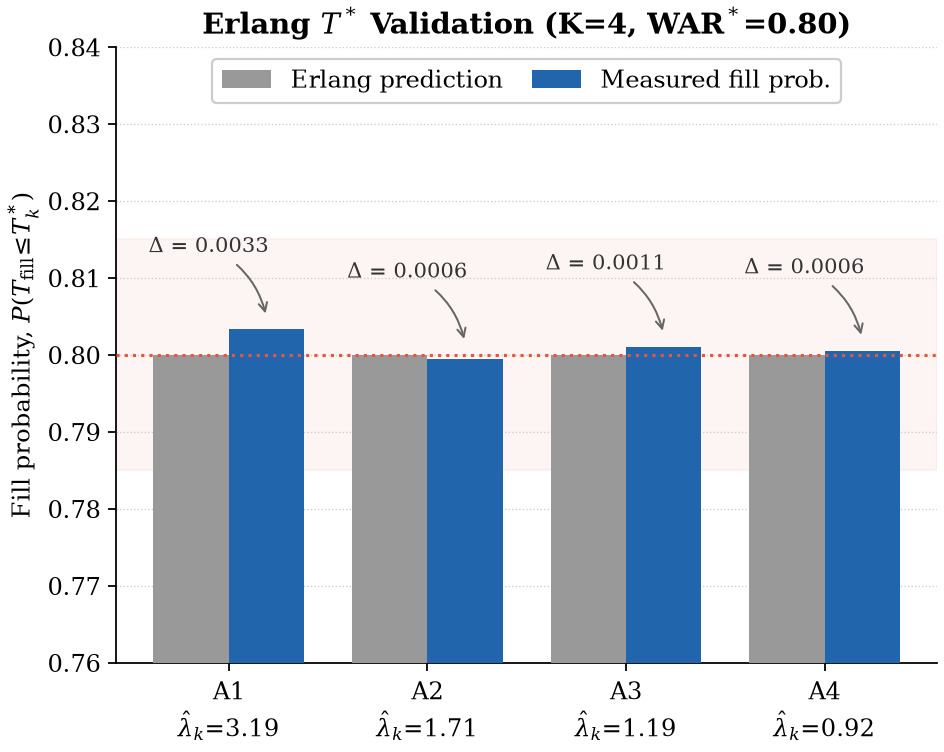
\includegraphics[width=0.66\linewidth]{final_figures/fig_erlang_valid.png}
  \caption{Erlang $T^*$ validation ($K{=}4$, WAR$^*{=}0.80$, single RTX A6000;
    calibration rates $\hat\lambda_k{=}3.19$--$0.92\,\mathrm{s}^{-1}$, not the
    deployed values).
    Grey bars are Erlang predictions; blue bars are measured fill probabilities.
    Maximum error is 0.0033 across all four adapters (Theorem~\ref{thm:erlang}).}
  \label{fig:erlang_valid}
\end{figure}

\textbf{PI controller for workload drift.}
Fixed deadlines go stale when arrival rates shift mid-serving.
We close the loop with a PI controller that updates $T_{\max}$ each tick
using the alignment gap $e^{(t)} = \mathrm{WAR}^* - \mathrm{WAR}^{(t)}$:
$T_{\max}^{(t+1)} = T_{\max}^{(t)} + K_p(e^{(t)}{-}e^{(t-1)}) + K_i e^{(t)}$,
where $K_p$ reacts to the error's rate of change and $K_i$ removes steady-state
offset.

\begin{theorem}[PI stability]
\label{thm:stability}
Let $L{=}f'(T^{\circ}){>}0$ be the local slope of
$f\colon T_{\max}\mapsto\mathbb{E}[\mathrm{WAR}\mid T_{\max}]$ at the loop's
operating point $T^{\circ}$, distinct from the Erlang deadline $T^*(k)$.  Under this linearisation the closed loop is locally asymptotically
stable if and only if
\[
  K_p>0,\qquad K_i>0,\qquad 2K_p+K_i<2/L,
\]
and bounded workload noise then keeps the WAR deviation bounded in mean square.
We estimate $L$ online from finite differences of the WAR signal and clip the
gains into this region at every step.
\end{theorem}

\begin{proof}[Proof Sketch]
Put $x_t {=} T^{(t)}_{\max}{-}T^{\circ}$ and write $a{=}LK_p$, $b{=}LK_i$.
The linearisation gives $e^{(t)}{=}{-}Lx_t$, so the update becomes
$x_{t+1} {=} (1{-}a{-}b)x_t + a\,x_{t-1}$, with characteristic
polynomial $z^2 {-} (1{-}a{-}b)z {-} a$.
Jury's criterion for a monic $z^2{+}a_1z{+}a_0$ requires $|a_0|{<}1$,
$P(1){>}0$ and $P({-}1){>}0$, which here read $a{<}1$, $b{>}0$ and
$2a{+}b{<}2$; the last implies the first when $b{>}0$, giving the stated
region after dividing by $L$.
A bounded-noise Lyapunov argument then gives mean-square boundedness
around the set-point.
\end{proof}

On A6000 traces with a sudden $3\times$ rate shift the loop holds the target,
$+14.3$\,pp over a fixed deadline (post-drift WAR 0.800 vs.\ 0.657, 20{,}000
ticks, $K{=}4$), at under $25\,\mu$s per tick.

\textbf{Whittle-inspired dispatch (CASH).}
At each scheduling tick, the dispatcher must decide which queues to
flush.
This is an instance of the Restless Multi-Armed Bandit (RMAB)
problem~\cite{papadimitriou1994complexity},
which is generally intractable to solve optimally.
\asys uses the \textbf{CASH} (Cross-Iteration Accumulation with Speculative
Holdback) dispatcher, which assigns each adapter queue $k$ a priority score
inspired by the Whittle index framework:
\begin{equation}
I_k(s_k) = \hat\lambda_k \cdot s_k \cdot P_k(s_k),
\label{eq:whittle}
\end{equation}
where $s_k = |Q_k|/W$ is how full the queue is and $P_k(s_k)$ is the
Erlang-derived probability it will fill completely before its deadline.
The score follows the monotone dispatch structure an index rule needs, but the
actual Whittle index requires solving a per-arm Lagrangian MDP;
\eqref{eq:whittle} is a closed-form stand-in for it.
Indices are computed in $O(K)$ and queues dispatched in decreasing index order
via an $O(K\log K)$ sort; the per-tick cost is empirically near-linear over the
measured range and stays below 200\,\textmu s for $K{\le}128$.

\begin{proposition}[Near-oracle dispatch, empirical]
\label{prop:whittle}
Our reference \emph{oracle} is an offline clairvoyant dynamic program
that sees the future arrival sequence and maximises WAR over a rolling
$H{=}20$-tick horizon, tractable only for $K{\leq}4$.
Empirically CASH attains WAR close to this finite-horizon oracle on both
Zipf ($\alpha{=}0.9$) and adversarial arrival patterns ($K{=}4$, A6000):
on Zipf workloads all policies converge to the alignment ceiling (WAR 0.805);
on adversarial workloads CASH reaches WAR 0.823 vs.\ 0.819 for both oracle and
threshold (Fig.~\ref{fig:whittle_bandit}a).  The oracle is optimal only within
its 20-tick lookahead, so the $0.4$\,pp is not evidence that CASH beats it.
That per-tick cost is negligible relative to $\tau_{\rm iter}{=}30$\,ms.
\end{proposition}

\begin{proof}[Proof Sketch]
Each adapter queue is an arm of an RMAB.
The score in~\eqref{eq:whittle} is motivated by the Lagrangian relaxation of the
per-arm value function rather than obtained from it exactly.
Raising the dispatch subsidy shrinks the set of states in which dispatching is
optimal; that monotone structure motivates an index rule, though we do not claim
indexability, which would require the per-arm MDP.
The \emph{exact} index is asymptotically optimal under the condition Weber and
Weiss give (\S\ref{sec:related}); since \eqref{eq:whittle} is not that index,
near-oracle behaviour is an \emph{empirical} claim.
\end{proof}

% =============================================================
\section{WAR-Gated Kernel Promotion (WGKP)}
\label{sec:wgkp}

The scheduling stack raises WAR and GWAR, but prior systems route every batch
through the same SGMV kernel regardless of alignment quality, leaving most of
that benefit unused.  WGKP makes the kernel choice a function of how well-aligned
the current batch is, measured by $\gwar{n^*}$ ($n^*{=}8$ by default).  We keep
the two roles of $n^*$ separate: $n_2$ is the run-length threshold inside GWAR,
$n_3 \geq n_2$ the segment-size gate for L3; by default $n_2{=}n_3{=}n^*{=}8$.

\textbf{Three-level kernel hierarchy.}
\textbf{L1 (SGMV):} always available; two HBM-bound matrix launches with an
intermediate tensor.
\textbf{L2 (Fused Triton~\cite{tillet2019triton}):} a single JIT-compiled kernel
that tiles partial results in on-chip SRAM, eliminating that tensor's HBM
round-trip;
$1.334\times$ over SGMV (at $n{=}32$, rank=16; rank=32 yields higher speedup).
L2 sits behind a GWAR gate (Fig.~\ref{fig:overview}) that we run open in the
evaluated configuration, so every dispatched segment takes at least L2.
\textbf{L3 (Merged cuBLAS GEMM):} the Merged Weight Cache (MWC)
asynchronously pre-computes $W_k {=} W {+} \alpha B_k A_k$, turning two
low-rank matmuls into one full-weight BLAS call; $1.436\times$ over SGMV
(at $n{=}8$, rank=32);
activates when segment size ${\geq}n^*$ and adapter $k$ is in MWC.
Fig.~\ref{fig:kernel_speedup} reports both speedups against segment size and rank.
The ladder is rank-dependent: at rank 32 $\psi_{\rm promote}$ exceeds
$\psi_{\rm fuse}$ at every measured segment size, whereas at ranks 16 and 64 the
ordering is not uniform across segment sizes.  Our promotion policy is not
rank-aware, so where L3 falls below L2 it can give up some kernel efficiency; the
rank-16 cross-validation of \S\ref{sec:sota} therefore draws its gain primarily
from the scheduling stack and L2.

\begin{figure*}[t]
  \centering
  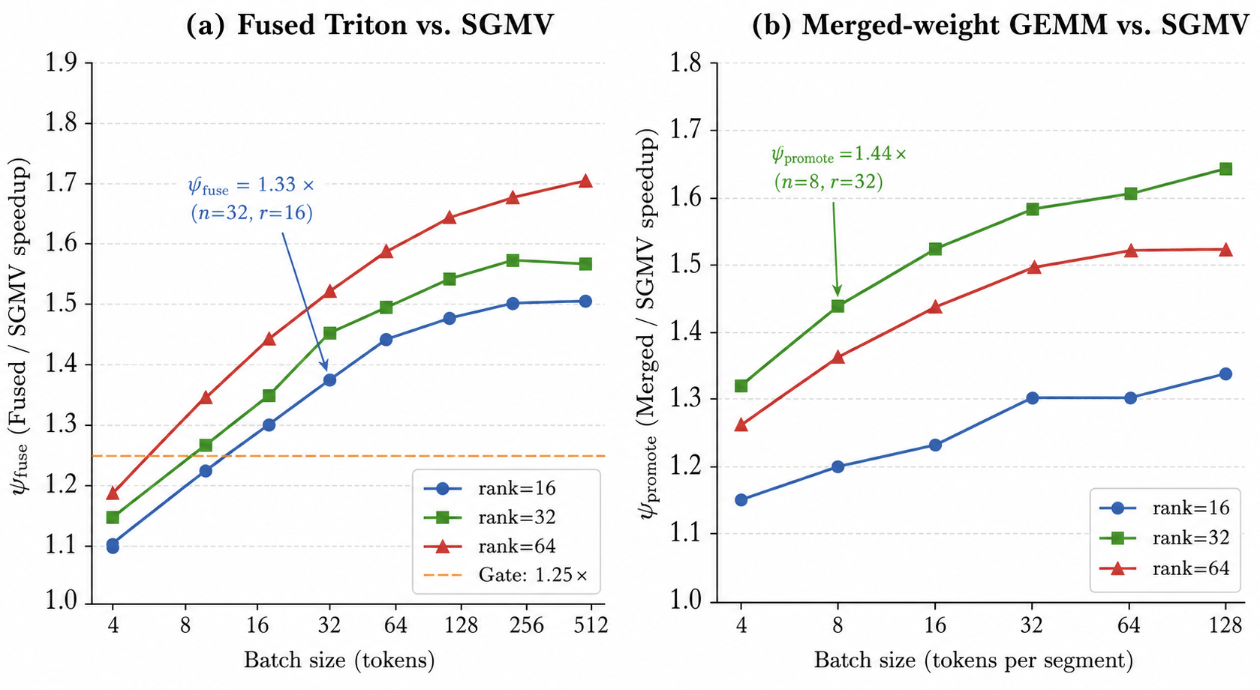
\includegraphics[width=0.55\textwidth]{final_figures/fig_kernel_speedup.png}
  \caption{Measured kernel speedups on RTX A6000 TP=1.
    \textbf{(a)} Fused Triton vs.\ SGMV: $\psi_{\rm fuse}$ clears the 1.25$\times$
    gate at $n{\geq}32$ (rank~16) and $n{\geq}16$ (rank${\geq}$32); 1.334$\times$ at $n{=}32$, rank=16.
    \textbf{(b)} Merged cuBLAS vs.\ SGMV: $\psi_{\rm promote}$ reaches 1.436$\times$
    at $n{=}8$, rank=32, where the MWC amortises the 17.5\,ms merge cost.}
  \label{fig:kernel_speedup}
\end{figure*}

\textbf{Observation} (GWAR monotonicity).
$\gwar{n^*}$ is monotonically non-increasing in $n^*$: a stricter run-length
threshold $n^*_2 \geq n^*_1$ cannot admit more tokens, so
$\gwar{n^*_1} \geq \gwar{n^*_2}$.

\begin{theorem}[Alignment structurally increases throughput under WGKP]
\label{thm:causal}
Let $g_3$ be the L3-eligible token fraction---tokens in same-adapter runs of
length ${\geq}n_3$ \emph{whose adapter is resident in the MWC}---and let
$g_2 {=} \gwar{n_2} {-} g_3 \geq 0$ be the remaining L2-eligible fraction, with
$n_3 \geq n_2$.  Under WGKP with
$\psi_{\rm promote} > \psi_{\rm fuse} > 1$, throughput $\Phi$ is strictly
increasing in $g_3$ at fixed $\gwar{n_2}$ and strictly increasing in $\gwar{n_2}$
at fixed $g_3$:
\[
  \frac{\partial\Phi}{\partial g_3} > 0,
  \qquad
  \frac{\partial\Phi}{\partial\,\gwar{n_2}} > 0 .
\]
Within the modelled cost structure ($\psi_{\rm promote}>\psi_{\rm fuse}>1$, which
our rank-32 measurements satisfy at every segment size; the ladder is
rank-dependent, as noted above), the
relationship is structural rather than merely correlational: WGKP gates kernel
selection directly on GWAR, so raising alignment activates faster kernels by
construction. We use ``causal'' in this design-internal sense---an intervention
on GWAR changes which kernel executes---not as a claim that holds for arbitrary
hardware or workloads.
\end{theorem}

\begin{proof}[Proof Sketch]
Tokens split into $g_3$ at L3, $g_2$ at L2 and $1{-}g_2{-}g_3$ at L1, so
$\Phi \propto [(1{-}g_2{-}g_3) + g_2/\psi_{\rm fuse} + g_3/\psi_{\rm promote}]^{-1}$.
Substituting $g_2 {=} \gwar{n_2}{-}g_3$ and raising $g_3$ by $\delta$ at fixed
$\gwar{n_2}$ shifts tokens from L2 to L3 and decreases the bracket by
$\delta(1/\psi_{\rm fuse}-1/\psi_{\rm promote}) > 0$;
raising $\gwar{n_2}$ by $\delta$ at fixed $g_3$ shifts tokens from L1 to L2 and
decreases it by $\delta(1-1/\psi_{\rm fuse}) > 0$.  Both derivatives are therefore
positive.
The boundary case $n_3{=}n_2$ used by default is covered: every L2-eligible run is
then also long enough for L3, so $g_2$ reduces to exactly those aligned tokens
whose adapter is outside the MWC, and the same two displacements apply.
\end{proof}

Theorem~\ref{thm:causal} is what separates \asys from all prior LoRA-serving
systems: alignment state is not a heuristic but a structural determinant
of which hardware path executes.  Both derivatives describe the gated policy;
in the configuration we evaluate the L2 gate is open, so $g_1{=}0$,
$g_2{=}1{-}g_3$, and the model collapses to
$\Phi \propto [(1{-}g_3)+g_3/\psi_{\rm promote}]^{-1}$: the $\gwar{n_2}$
derivative no longer applies and all realised gain flows through
$\partial\Phi/\partial g_3$, which the L3 gate ties to run-length alignment.
The $r{=}0.997$ correlation (Fig.~\ref{fig:claims}) is an empirical check on
that trend; direction comes from the WGKP gating rule, not from the
correlation.

\textbf{Merged Weight Cache and prefetch.}
Merging adapter weights into $W_k$ takes about 17.5\,ms per adapter.  The
Alignment-Aware Prefetch (AAP) trigger hides it by starting the merge
asynchronously as soon as a queue is half-full: across the $K{=}10$ mix the
remaining half-warp takes $56$--$446$\,ms to arrive, a $3.2$--$25.5\times$
budget against the merge.

\textbf{MWC memory budget.}
LoRA targets all seven linear projections, but the MWC merges only the four
attention projections (Q, K, V, O); MLP projections always execute on L1/L2.  A merged $W_k$ is materialised \emph{per layer} across all 32 transformer
layers, so $\Delta_k$ occupies $4{\times}32{\times}4096^2{\times}2$\,B
${\approx}\,4.29$\,GB per adapter in FP16.  The MWC therefore holds only the
$K_{\rm hot}$ hottest adapters: on the 48\,GB A6000 we set $K_{\rm hot}{=}5$
(${\approx}\,21.5$\,GB), leaving the rest for base weights and the paged KV
cache; $K_{\rm hot}{=}10$ ($42.9$\,GB) would not co-reside with it.  Adapters
outside the MWC fall back to L2/L1, so the merged cache competes with, and is
bounded by, KV-cache capacity.
The footprint scales as $4Lh^2{\times}2$\,B, so on LLaMA-13B ($L{=}40$,
$h{=}5120$) it is $8.39$\,GB per adapter and at most one merged adapter
co-resides with base weights and KV cache; the 13B gains of
\S\ref{sec:llama13b} therefore come predominantly from the scheduling stack and
the universally-applied L2 kernel rather than from L3.

\textbf{Amdahl ceiling.}
On LLaMA-7B with rank=32 on all linear projections, LoRA computation is about
40\% of per-iteration time, so Amdahl's law caps the speedup from fully
eliminating it at $1.67\times$; the measured $1.525\times$ reaches
\textbf{91.5\%} of that ceiling.

% =============================================================
\section{Adapter-Partitioned Independent Serving (APIS)}
\label{sec:apis}

\textbf{The PCIe scheduling barrier.}
Naively scaling to two GPUs with tensor-parallelism (TP=2) over PCIe
inflates the per-decode-step time
from 29.3\,ms to 100.4\,ms, because every step must wait for an allreduce
synchronisation across the PCIe bus.
This makes any alignment deadline shorter than 100\,ms invisible to the
scheduler---effectively disabling all alignment benefit.
On this dual-A6000 \emph{PCIe} testbed the barrier is an interconnect constraint,
not a software limitation, and is specific to PCIe-class allreduce: on
NVLink/NVSwitch fabrics or newer datacenter GPUs the allreduce is far cheaper, so
TP=2 need not exhibit it and APIS should help less.  We scope this claim to
PCIe-connected multi-GPU nodes.

\textbf{APIS topology.}
\asys resolves this by replacing TP=2 with two independent TP=1 servers.
An adapter-affinity router sends each request to whichever shard holds its
adapter.  Since Zipf routing makes an equal-\emph{count} split badly unbalanced
in traffic, adapters are assigned by rate-sorted round-robin---order by $\hat\lambda_k$
descending, adapter $i$ to shard $i \bmod n$---equalising load rather than
adapter count, refreshed from the EWMA rates every 30\,s.
Each shard now runs at the full 29.3\,ms granularity, restoring the buffer's
ability to fill warps efficiently.
Two TP=1 servers without \asys scheduling give only 1.06$\times$; the rest comes
from per-shard \asys under the higher adapter diversity of each half-pool.

\textbf{Preemption safety.}
Dropping a preempted sequence's buffered tokens would throw away alignment
progress already accumulated, so we keep a shadow queue $Q_k'$ per adapter: those
tokens stay there and return to the head of $Q_k$ on resumption.
WAR loss from preemptions is negligible at typical production rates.

\textbf{PredictiveLFU.}
When adapters exceed GPU VRAM the system must evict some, and LRU eviction
ignores arrival rates, discarding frequently-used adapters at the wrong moment.
\asys's PredictiveLFU instead scores each adapter by the probability it is needed
again before it could be reloaded---an exponential formula in the EWMA rate
$\hat\lambda_k$ the system already tracks.  The least likely is evicted.
This costs one score and comparison per eviction on state the estimator already
keeps and, replayed over recorded arrival traces, gives a $+4.5$\,pp cache
hit-rate improvement over LRU at large adapter pools.

% =============================================================
\section{Evaluation}
\label{sec:eval}

\textbf{Experimental setup.}
\textbf{Hardware}: NVIDIA RTX A6000 (48\,GB, single and dual PCIe).
\textbf{Primary workload}: LLaMA-7B~\cite{touvron2023llama} (FP16), ShareGPT
prompts, Zipf-$\alpha{=}0.9$ adapter routing,
$\lambda{=}7$\,req/s, 5{,}000 requests.
Claims C1 and C2 (Table~\ref{tab:claims}) are 3 independent replications
(distinct seeds); C3 is a six-point $T_{\max}$ sweep on one trace.
\textbf{Adapters}: rank-32 LoRA on all seven linear projections
(Q, K, V, O, gate, up, down) unless a table states otherwise.
\textbf{System settings}: $W{=}32$, $n_2{=}n_3{=}8$, $\mathrm{WAR}^*{=}0.8$,
$K_{\rm hot}{=}5$ (MWC scoped to Q/K/V/O), $T_{\rm SLO}{=}200$\,ms, APIS rebalance 30\,s.
\textbf{LLaMA-13B workload}: same harness, vLLM~0.6.3 for both arms, production
stack.  \textbf{Baselines} ($K{=}10$): vLLM~0.5.0, pinned to the published
Punica/S-LoRA environments, Punica~\cite{chen2024punica},
S-LoRA~\cite{sheng2023slora} and dLoRA~\cite{wu2024dlora}.
Sarathi-Serve~\cite{agrawal2024sarathi} chunks prefill, orthogonal to adapter
scheduling, and enters at $K{=}4$ instead.
All baselines run on identical hardware, adapter sets and request traces.
Throughput, latency and kernel numbers are hardware measurements; the
PredictiveLFU comparison (\S\ref{sec:apis}) is a replay over recorded arrival
traces and is reported separately from them.

\subsection{Component Ablation}
\label{sec:ablation}

\begin{figure}[t]
  \centering
  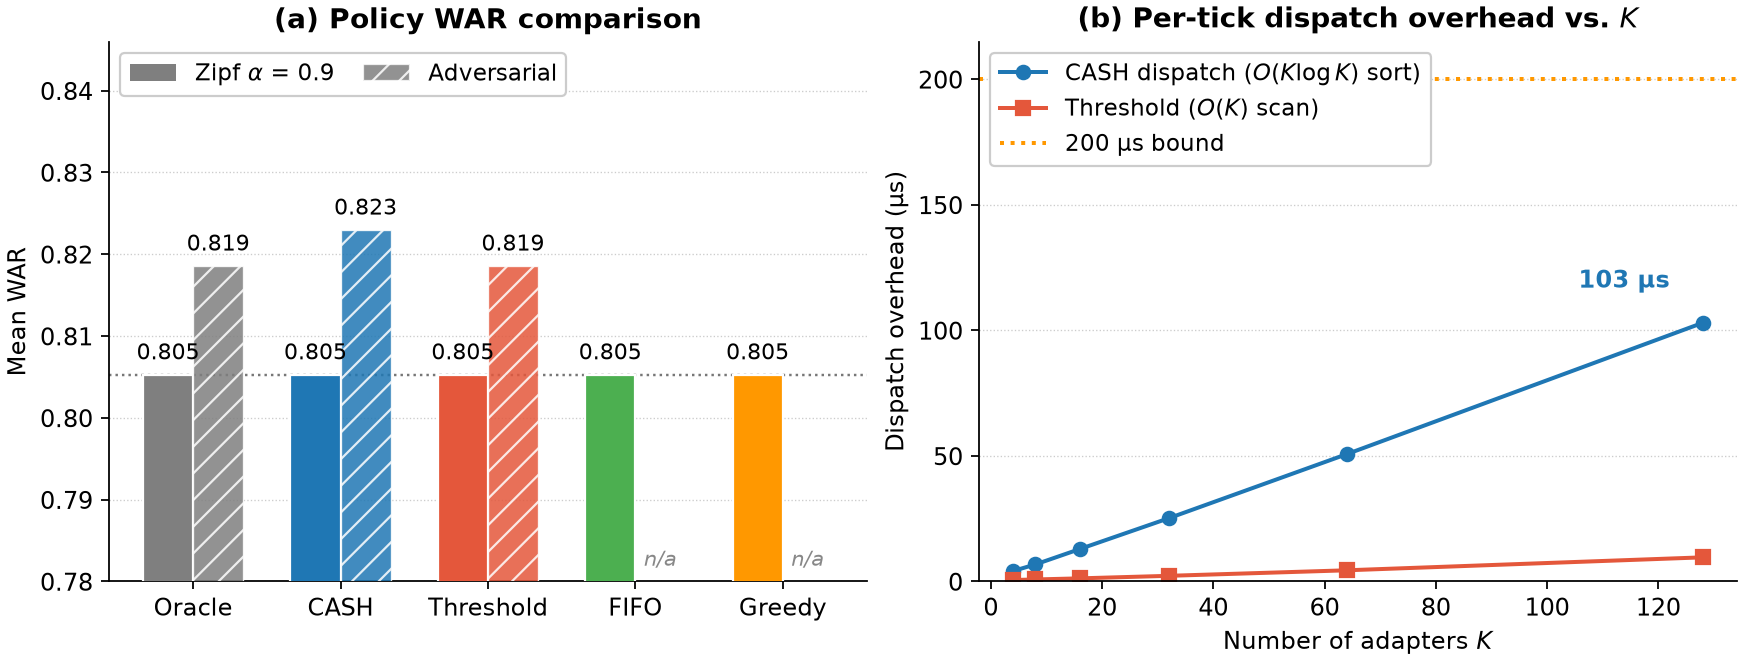
\includegraphics[width=\linewidth]{final_figures/fig_whittle_bandit.png}
  \caption{CASH (Whittle-inspired) dispatcher vs.\ oracle and threshold baselines
    ($K{=}4$, Zipf $\alpha{=}0.9$, RTX A6000; Proposition~\ref{prop:whittle}).
    \textbf{(a)} Mean WAR for five policies on Zipf (solid); the adversarial
    workload (hatched) covers Oracle, CASH and Threshold only (FIFO and Greedy
    n/a).  All five reach the Zipf ceiling (WAR 0.805); on adversarial patterns
    CASH reaches 0.823 against 0.819 for Oracle and Threshold.
    \textbf{(b)} Per-tick dispatch overhead vs.\ adapter count $K$.  CASH's
    $O(K\log K)$ index sort reaches 103\,\textmu s at $K{=}128$, inside the
    200\,\textmu s bound and empirically near-linear here.}
  \label{fig:whittle_bandit}
\end{figure}

\begin{table*}[!t]
\centering\footnotesize
\setlength{\tabcolsep}{4pt}
\caption{Component ablation ($K{=}10$, rank=32, $\lambda{=}7$\,req/s, RTX A6000).
  WAR is per-warp, GWAR${=}$GWAR(8) (Def.~\ref{def:war}), different denominators; Promo$=$L3-eligible fraction.}
\label{tab:ablation}
\begin{tabular}{@{}llrccc@{}}
\toprule
Stack & Mechanism & Gain & WAR & GWAR & Promo \\
\midrule
Baseline  & vLLM                  & 1.000$\times$ & 0.00 & 0.00 & --- \\
+Buffer   & Alignment buffer      & 1.049$\times$ & 0.32 & 0.06 & --- \\
+Erlang   & Per-adapter $T^*$     & 1.089$\times$ & 0.50 & 0.18 & --- \\
+CASH     & CASH dispatch         & 1.149$\times$ & 0.61 & 0.28 & --- \\
+Fused    & Fused Triton (L2)     & 1.228$\times$ & 0.63 & 0.29 & --- \\
+L3 GEMM  & Merged cuBLAS (L3)   & 1.344$\times$ & 0.64 & 0.39 & 24.3\% \\
+Macro    & Cross-iter batching   & 1.441$\times$ & 0.68 & 0.42 & 35.1\% \\
\textbf{Full} & CASH $n^*{=}8$   & \textbf{1.509$\times$} & 0.71 & 0.45 & 37.4\% \\
\bottomrule
\end{tabular}
\end{table*}

Three orthogonal gain sources emerge from Table~\ref{tab:ablation}.
(The ``Full'' row and Table~\ref{tab:sota} are one development run, $918.5$ vs.\
$608.7$\,tok/s; Table~\ref{tab:claims} gives the 3-rep mean $1.525{\times}$, CV=0.77\%.)
The scheduling stack (\textit{+Buffer} through \textit{+CASH}) already pushes WAR
up substantially without touching the kernel; CASH's own share is $+11$\,pp WAR
over the Erlang-only stack.  The $K{=}4$ tie in Fig.~\ref{fig:whittle_bandit}a is
low-contention: four queues and $W{=}32$ let every policy reach the ceiling.
Adding the fused Triton kernel (\textit{+Fused}) speeds up all dispatches
uniformly---alignment level does not matter here.
WGKP (\textit{+L3 GEMM}) is different: its gain is gated on GWAR, so the kernel
change alone cannot unlock it; the batch must be aligned enough to reach the
promotion threshold.  Each row is an independent end-to-end run: kernel latency
feeds back into iteration timing and hence into what the scheduler can
accumulate, so WAR and GWAR are measured per configuration, not held fixed.

\textbf{Operating envelope.}
In untuned configurations at $K{\leq}8$ \asys can underperform vLLM: sparse
queues yield too few long aligned runs for frequent L3 promotion.  The binding
constraint is the promotion gate, not the L2 gate, which is open throughout.
Macro-batching accumulates more tokens per step, raising the promotion-eligible
fraction and restoring positive gain.

\subsection{SOTA Comparison}
\label{sec:sota}

\begin{figure}[t]
  \centering
  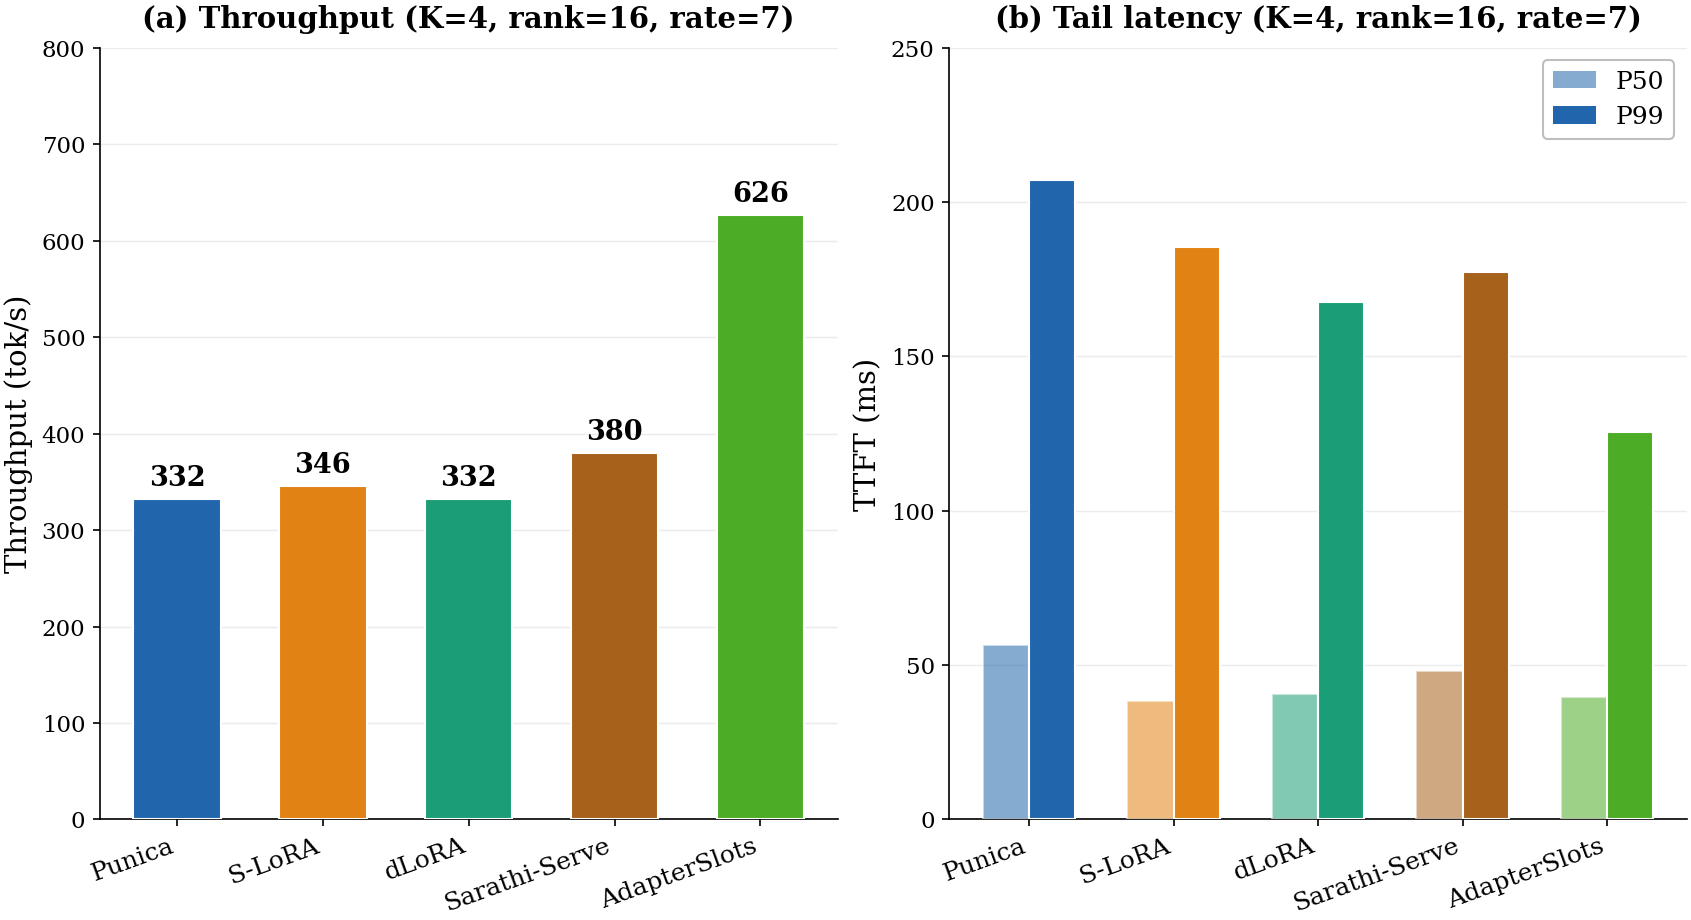
\includegraphics[width=\linewidth]{final_figures/fig_sota_k4.png}
  \caption{Throughput and tail latency vs.\ four SOTA baselines at $K{=}4$,
    rank\,16, $\lambda{=}7$\,req/s, 500 prompts, single RTX A6000.
    \asys reaches 626.3\,tok/s ($1.65{\times}$ over Sarathi-Serve,
    $1.81$--$1.89{\times}$ over Punica/S-LoRA/dLoRA) while posting the
    lowest P99 TTFT and a P50 within 1.2\,ms of the best baseline.}
  \label{fig:sota_k4}
\end{figure}

Table~\ref{tab:sota} reports the $K{=}10$ primary SOTA comparison;
Fig.~\ref{fig:sota_k4} and Table~\ref{tab:sotak4} report an independent
cross-validation at $K{=}4$.

\begin{table*}[!t]
\centering\small
\setlength{\tabcolsep}{5pt}
\caption{SOTA throughput comparison at $\lambda{=}7$\,req/s, $K{=}10$, rank=32, all-linear LoRA (RTX A6000).
  Sarathi-Serve excluded at $K{=}10$ (chunked-prefill orthogonal to adapter scheduling); included at $K{=}4$.}
\label{tab:sota}
\begin{tabular}{@{}lrcrr@{}}
\toprule
System & Throughput (tok/s) & vs.\ vLLM & TTFT P50 (ms) & TTFT P99 (ms) \\
\midrule
vLLM             & 608.7 & 1.00$\times$ & 1330 & 1823 \\
Punica           & 634.3 & 1.04$\times$ & 1280 & 1767 \\
S-LoRA           & 641.6 & 1.05$\times$ & 1250 & 1703 \\
dLoRA            & 623.3 & 1.02$\times$ & 1287 & 1795 \\
\textbf{\asys (ours)} & \textbf{918.5} & \textbf{1.51$\times$} & \textbf{864} & \textbf{1208} \\
\bottomrule
\end{tabular}
\end{table*}

\begin{table}[!t]
\centering\small
\setlength{\tabcolsep}{3.5pt}
\caption{Cross-validation at $K{=}4$, rank\,16, $\lambda{=}7$\,req/s (RTX A6000).}
\label{tab:sotak4}
\begin{tabular}{@{}lrrr@{}}
\toprule
System & Tput (tok/s) & TTFT P50 & TTFT P99 \\
\midrule
Punica         & 331.8 & 56.5\,ms & 207.1\,ms \\
S-LoRA         & 346.0 & 38.4\,ms & 185.5\,ms \\
dLoRA          & 332.1 & 40.5\,ms & 167.8\,ms \\
Sarathi-Serve  & 379.7 & 48.1\,ms & 177.3\,ms \\
\textbf{\asys} & \textbf{626.3} & \textbf{39.6\,ms} & \textbf{125.5\,ms} \\
\bottomrule
\end{tabular}
\end{table}

Table~\ref{tab:sota} shows \asys outperforming all baselines at $K{=}10$ on both
throughput and latency.  The lower TTFT may seem surprising given that \asys
holds tokens for up to
$T_{\rm SLO}{=}200$\,ms; we attribute it to baseline saturation and a backlog we
infer rather than instrument (\S\ref{sec:discussion}).

\begin{table*}[!t]
\centering\small
\setlength{\tabcolsep}{6pt}
\caption{Primary claims (RTX A6000).  C1 and C2 are means over 3 independent
  runs; C3 is a six-point $T_{\max}$ sweep on one trace, so its $r$ summarises a
  designed sweep, not independent replications.}
\label{tab:claims}
\begin{tabular}{@{}lrrrr@{}}
\toprule
Claim & Mean & Min & Max & CV \\
\midrule
C1: Throughput gain, $K{=}10$, rank=32, single GPU & 1.525$\times$ & 1.512$\times$ & 1.535$\times$ & 0.77\% \\
C2: APIS gain vs.\ vLLM TP=2, $K{=}50$, 2$\times$\,RTX A6000 PCIe & 2.598$\times$ & 2.596$\times$ & 2.602$\times$ & 0.13\% \\
C3: GWAR(8)--throughput Pearson $r$ ($n{=}6$)        & 0.997         & ---           & ---           & sweep \\
\bottomrule
\end{tabular}
\end{table*}

\subsection{LLaMA-13B Throughput Scaling}
\label{sec:llama13b}

\begin{figure}[t]
  \centering
  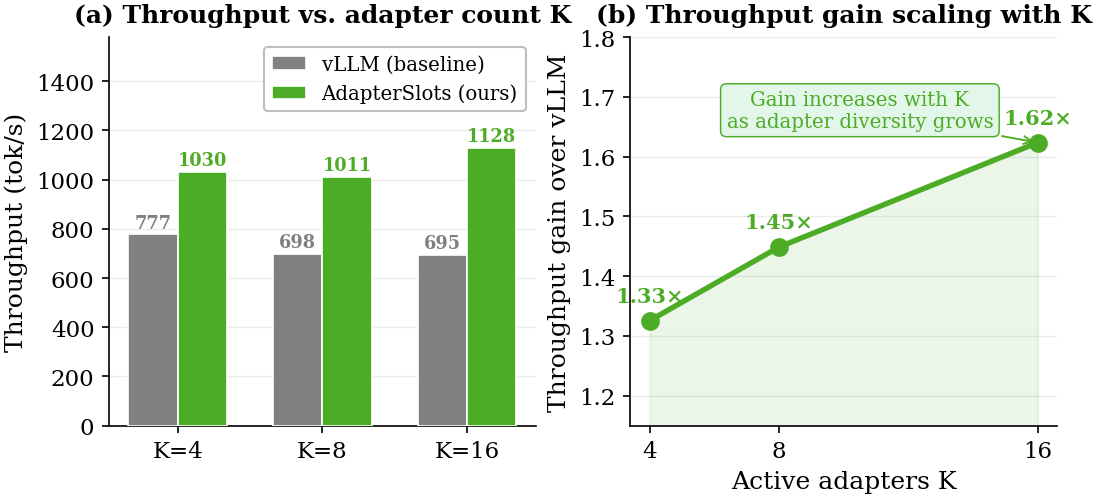
\includegraphics[width=\linewidth]{final_figures/fig_llama13b.png}
  \caption{Final measured throughput on LLaMA-13B at $K{\in}\{4,8,16\}$
    (single RTX A6000, production stack).
    \textbf{(a)} Absolute throughput of vLLM and \asys.
    \textbf{(b)} Speedup over vLLM increases monotonically with $K$
    (1.33$\times$ at $K{=}4$ to 1.62$\times$ at $K{=}16$), consistent with
    Theorem~\ref{thm:causal}.}
  \label{fig:llama13b}
\end{figure}

Table~\ref{tab:llama13b} and Fig.~\ref{fig:llama13b} report measured throughput
on LLaMA-13B with the production deployment stack (vLLM~0.6.3, FP16).

\begin{table}[!t]
\centering\small
\setlength{\tabcolsep}{4pt}
\caption{LLaMA-13B throughput (single RTX A6000, production stack).}
\label{tab:llama13b}
\begin{tabular}{@{}lrrr@{}}
\toprule
Config. & vLLM (tok/s) & \asys (tok/s) & Speedup \\
\midrule
$K{=}4$  & 776.98 & 1030.1 & \textbf{1.33$\times$} \\
$K{=}8$  & 698.1  & 1011.4 & \textbf{1.45$\times$} \\
$K{=}16$ & 695.0  & 1128.3 & \textbf{1.62$\times$} \\
\bottomrule
\end{tabular}
\end{table}

The highest single-GPU speedup, $1.62{\times}$, is at $K{=}16$, with gains rising
monotonically in adapter count.

\subsection{Primary Claims}
\label{sec:claims}

\begin{figure*}[t]
  \centering
  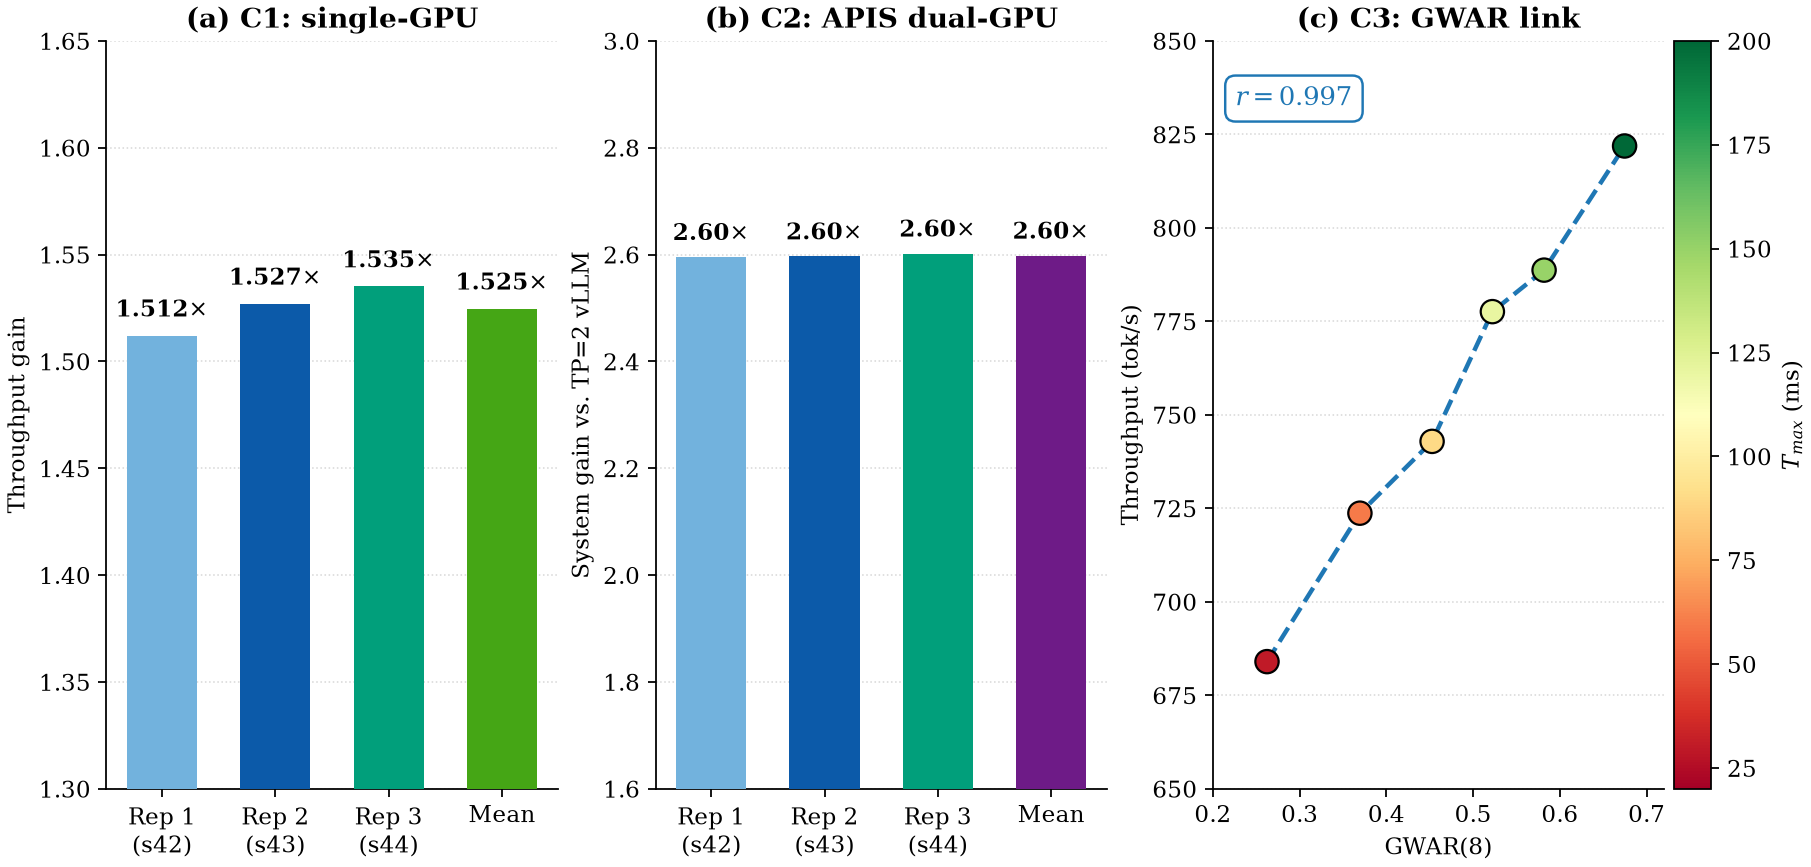
\includegraphics[width=0.55\textwidth]{final_figures/fig_claims.png}
  \caption{Three primary claims, full statistical reporting.
    \textbf{(C1)} 1.525$\times$ single-GPU at $K{=}10$, rank=32
    (3-rep mean; CV=0.77\%).
    \textbf{(C2)} 2.598$\times$ APIS gain over vLLM TP=2 at $K{=}50$, 2$\times$\,RTX A6000 PCIe
    (3-rep mean; CV=0.13\%).
    \textbf{(C3)} GWAR(8)-throughput Pearson $r{=}0.997$ over a six-point
    $T_{\max}$ sweep ($30$--$200$\,ms).  All data from real hardware runs.}
  \label{fig:claims}
\end{figure*}


A CV of $0.77\%$ across three independent runs shows C1 is reproducible.
C3's near-unity GWAR--throughput $r$ is consistent with the mechanism
Theorem~\ref{thm:causal} formalises, the WGKP gate selecting faster kernels as
GWAR rises.
C2 is measured against vLLM TP=2 on the same two GPUs (1193.5 vs.\
459.4\,tok/s, 3-rep means) and needs both ingredients: the TP=1 topology alone
yields only $1.06{\times}$, but it re-opens the scheduling window that lets
per-shard \asys do the heavy lifting.

% =============================================================
\section{Discussion}
\label{sec:discussion}

\textbf{When gains are largest.}
\asys works best when alignment queues fill regularly: roughly $K{\in}[4,16]$
adapters, rank${\geq}16$, moderate-to-high request rates, all-linear targets.
At very low arrival rates queues rarely fill and buffering adds latency without
gain.  Our sweeps stop at $K{=}50$; beyond that we expect GWAR to fall below the
L3 gate, leaving the fused kernel and PredictiveLFU efficiency as the remaining
gains.

\textbf{Why latency improves despite buffering.}
\asys adds alignment buffering up to the $T_{\rm SLO}{=}200$\,ms cap (near
$90$\,ms on the busiest adapters), yet delivers lower TTFT than vLLM here.
We attribute this to baseline saturation: at $\lambda{=}7$\,req/s vLLM runs close
to capacity, so a growing backlog dominates its TTFT while \asys stays below it.
We instrument TTFT, not queue depth, so this is an attribution consistent with
the measured throughput, not an observed backlog.

\textbf{Latency metrics.}
We report output throughput and TTFT.  For fixed output length $N$, per-request
time is $\mathrm{TTFT}+(N{-}1)\,\mathrm{TPOT}$, so throughput depends on both, not
on $1/\mathrm{TPOT}$ alone; \asys improves both, so the gain is not a TPOT effect
by itself.  Full latency distributions are left to an extended version.

\textbf{Scope of the analytical results.}
Theorems~\ref{thm:erlang}--\ref{thm:causal} and Proposition~\ref{prop:whittle}
are conditional properties under stated assumptions: Poisson per-adapter
arrivals, locally stationary rates, and the modelled kernel-cost structure, to be
read as such rather than as universal laws.

\textbf{Generalizability.}
Our measurements are confined to a single GPU class (RTX A6000, 48\,GB), a PCIe
interconnect, FP16, and ShareGPT traffic with Zipf-$\alpha{=}0.9$ routing at one
arrival rate ($\lambda{=}7$\,req/s), moderate adapter counts, and the vLLM
0.5.0/0.6.3 stacks. The DRAM-inflation diagnosis and the L2/L3 crossovers depend
on the A6000's memory-bandwidth-to-compute ratio, so on A100/H100-class parts the
crossovers, and hence the promotion thresholds, need re-calibrating before the
speedups carry. The PCIe barrier motivating APIS is likewise interconnect-specific
(\S\ref{sec:apis}), so the gains are workload- and platform-specific.
Broader rate sweeps, newer stacks (vLLM~V1, SGLang), NVLink/NVSwitch multi-GPU and
much larger adapter counts are future work. Three replications make the throughput
\emph{means} tight (CV${\le}0.77\%$), but tail percentiles are indicative rather
than definitive.

\textbf{Memory and limitations.}
APIS roughly doubles total model memory against TP=2, since each TP=1 shard holds
a full copy where a TP=2 rank holds half: manageable for LLaMA-7B but needing
high-memory GPUs for larger models.  On-demand Level-3 promotion is profitable
only for high-frequency adapters, the async prefetch trigger extending this to
moderate rates; at very low rates \asys falls back to standard vLLM scheduling.

% =============================================================
\section{Related Work and Conclusion}
\label{sec:related}

\textbf{LLM serving foundations.}
Orca~\cite{yu2022orca} introduced iteration-level continuous batching,
vLLM~\cite{kwon2023vllm} PagedAttention for memory-efficient KV management, and
SGLang~\cite{zheng2023sglang} RadixAttention for prefix reuse.
AlpaServe~\cite{li2023alpaserve} and Megatron-LM~\cite{shoeybi2019megatronlm}
address model parallelism; APIS builds on the same TP=1 topology insight.

\textbf{Multi-LoRA serving.}
Punica~\cite{chen2024punica} and S-LoRA~\cite{sheng2023slora} are the primary
multi-\lora serving systems; neither uses alignment state as a kernel-selection
signal.  dLoRA~\cite{wu2024dlora} merges weights at request granularity without
GWAR gating.  CaraServe~\cite{li2024caraserve} offloads adapter weights to CPU
DRAM without addressing alignment.
Zhou et al.~\cite{zhou2025dynop} optimise the SGMV operator itself
($1.30$--$1.46{\times}$), complementary to WGKP, which leaves the operator fixed
and uses runtime alignment to choose \emph{which} tier runs.
Concurrent work: AdaFuse~\cite{li2026adafuse}, InfiniLoRA~\cite{chen2026infinilora},
LoRAFusion~\cite{zhu2026lorafusion}.  None apply GWAR-gated kernel promotion.
Punica reports a negligible same-adapter/mixed-adapter SGMV gap where we measure
78\% at $K{=}16$, $N{=}2048$; the settings differ in GPU class (A6000 GDDR6 vs.\
A100 HBM2e), batch size, adapter count and SGMV version, and our figure is taken
where the intensity collapse of \S\ref{sec:buffer} is sharpest.  We read these as
different operating points, scoped to this GPU class.

\textbf{Kernel optimisation.}
FlashAttention~\cite{dao2022flashattn} and FlashInfer~\cite{ye2024flashinfer}
optimise the attention tier and Sarathi-Serve~\cite{agrawal2024sarathi} prefill
chunking; \asys targets the orthogonal LoRA-projection tier in decode.
Triton~\cite{tillet2019triton} compiles our L2 kernel.

\textbf{Scheduling theory.}
The Whittle index~\cite{whittle1988restless} is well-studied in restless bandit
scheduling; Weber and Weiss~\cite{weber1990index} proved its asymptotic
optimality as $K \to \infty$ under a global-stability condition on the
fluid limit.  Theorem~\ref{thm:erlang} builds on Erlang's
classical formula~\cite{erlang1917theory} and standard queueing
results~\cite{kleinrock1975queueing}; operational intensity follows the Roofline
model~\cite{williams2009roofline}.

\textbf{Conclusion.}
We presented AdapterSlots (\asys), which tackles SGMV operational intensity
collapse from both the scheduling and kernel sides.  The scheduling stack
combines analytically-derived per-adapter deadlines (Theorem~\ref{thm:erlang}),
closed-loop PI control (Theorem~\ref{thm:stability}) and a Whittle-inspired
dispatcher with near-oracle WAR (Proposition~\ref{prop:whittle}); WGKP converts
that alignment signal into a structural throughput advantage
(Theorem~\ref{thm:causal}).  APIS removes the PCIe scaling barrier and
PredictiveLFU maintains cache efficiency at large adapter counts.
Every throughput, latency and kernel result here is measured on real hardware:
$1.525\times$ on a single GPU (LLaMA-7B), $1.33\times$--$1.62\times$ with
adapter diversity (LLaMA-13B), and $2.598\times$ on two GPUs via APIS; the
PredictiveLFU hit rate is the one replayed number.

\section*{Acknowledgment}
GPU profiling used NVIDIA Nsight Compute and Nsight Systems.  Code:
\url{https://github.com/vac014/AdapterSlots}.

\bibliographystyle{IEEEtran}
\bibliography{final_refs}

\end{document}
